\documentclass[11pt,usenames,dvipsnames]{beamer}
\usetheme{Madrid}
\usepackage{lmodern}
\usepackage{xcolor}



\usepackage[utf8]{inputenc}
\usepackage[english]{babel}
\usepackage{amsmath}
\usepackage{amsfonts}
\usepackage{amssymb}
\usepackage{graphicx}
\usepackage{tikz}



\setbeamercolor{block title alerted}{fg=Red, bg=Salmon!50!White}
\setbeamercolor{block body alerted}{bg=Salmon!20!White}


\setbeamercolor*{block title example}{fg=black, bg=Goldenrod}
\setbeamercolor{block body example}{bg=Goldenrod!30!White}

\setbeamercolor*{block title}{fg=White, bg=ForestGreen}
\setbeamercolor{block body}{bg=LimeGreen!30!White}

\setbeamertemplate{footline}{
\begin{flushright}
\Large\insertframenumber
\end{flushright}}
\setbeamertemplate{navigation symbols}{}
\author{Presentation by Phil Trommer}
\title{A Machine Learning Perspective on Predictive Coding with PAQ by Knoll \& de Freitas}
%\setbeamercovered{transparent} 
%\setbeamertemplate{navigation symbols}{} 
%\logo{} 
%\institute{} 
%\date{} 
%\subject{} 

% Inserts Section Introduction Slide
\AtBeginSection[] {
	\begin{frame}
		\frametitle{\insertsectionhead}
		\tableofcontents[currentsection,hideothersubsections]
	\end{frame}
}


\newcommand{\defText}[1]{\textcolor{Red}{#1}}





\colorlet{beamer@blendedblue}{ForestGreen}
\begin{document}



\begin{frame}
\titlepage
\end{frame}


\begin{frame}{Overview}
\tableofcontents
\end{frame}


\section{Introduction to PAQ}


\begin{frame}{Introduction to PAQ}
	\begin{block}{What is PAQ8}
			\begin{itemize}
				\item What is it?
				\item How does it work?
				\item What makes it so famous?
			\end{itemize}
	\end{block}
\end{frame}

\begin{frame}{Introduction to PAQ}
	\begin{exampleblock}{Matt Mahoney}<1->
	\begin{minipage}[b]{0.70\linewidth}
		\begin{itemize}
			\item Born 1955
			\item Recieved Ph.D in computer science at Florida Tech in 2003
			\item Released PAQ1 on January 6, 2002
		\end{itemize}
	\hfill
	\end{minipage}
	\begin{minipage}[b]{0.28\linewidth}
		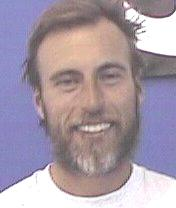
\includegraphics[scale=1.5]{files/matt.jpg}
	\end{minipage}
	\end{exampleblock}
	
	\begin{alertblock}{What is PAQ?}<2->
		\begin{itemize}
			\item A lossless, open-source compression algorithm
			\item Brings high perfomance at the cost of increased memory usage and time consumption
			\item Related to PPM, is envisioned as PPMs improvement
		\end{itemize}
	\end{alertblock}
\end{frame}

\begin{frame}{Introduction to PAQ}
	\begin{exampleblock}{Principles of PAQ}
	
		\begin{itemize}
			\item Modeling combined with adaptive arithmetic encoding
			\item Open to additions and improvements
			\item Improves perfomance of PPM by including several predictors (i.e. models of data) 
			\item Combines the result of the predictors 
		\end{itemize}
	\end{exampleblock}

\end{frame}

\begin{frame}{Introduction to PAQ}
	\begin{block}{Exemplary Predictors}<1->
	\visible<2->{The order-$n$ context predictor
		\begin{itemize}
			\item Examines the last $n$ bits and counts the 1's and 0's
			\item Estimates probability whether next bit is 1 or 0 like PPM
		\end{itemize}	
		}		
	\visible<3->{
	The sparse context predictor
		\begin{itemize}
			\item 	Context consists of a specific amount of non-contiguous bytes before the current bit 
		\end{itemize}
		}
	\end{block}
	
	\begin{exampleblock}{PAQ \& Predictors}<3->
		\begin{itemize}
			\item PAQ encoder looks at the beginning of input file for deciding which predictors are used
			\item Ways to combine predictions change through with the different versions
		\end{itemize}

	\end{exampleblock}
	
\end{frame}

\section{PAQ8L}
\begin{frame}{PAQ8L}
	\begin{exampleblock}{PAQ8 - What's new?}<1->
		\begin{itemize}
			\item Predictors don't produce a pair of bit counts anymore\\
			$\hookrightarrow$ those counts get weighted and normalized into the interval $[0,1]\subset\mathbb{R}$
			\item Instead  each predictor already outputs a probability
			\item \textit{paq8l} is a stable version of paq8, released by Matt Mahoney
		\end{itemize}
	\end{exampleblock}
	
		\begin{alertblock}{PAQ8L - Machine Learning Perspective}<2->
		\begin{itemize}
			\item paq8l is the version of PAQ used by \textit{Byron Knoll \& Nando de Freitas}
			\item They try to show the possibilities of PAQ beyond data compression
		\end{itemize}
	\end{alertblock}
\end{frame}

\subsection{Architecture}
\begin{frame}{Architecture}


	\begin{exampleblock}{Architecture of PAQ8}<1->
		\begin{itemize}
			\item Uses weighted combination of predictions from Large number of models
			\item Allows no-contiguous context matches
			\item paq8l uses \textbf{552} prediciton models
			\item Combines the output of them into a single one\\
			$\hookrightarrow$ Passes this through an \textit{adaptive probability map} (APM) before using the arithmetic coder
		\end{itemize}
	\end{exampleblock}
	\hfill
	
	\visible<2->{
	\begin{figure}[H]
		\centering
		\resizebox{0.95\textwidth}{!}{
			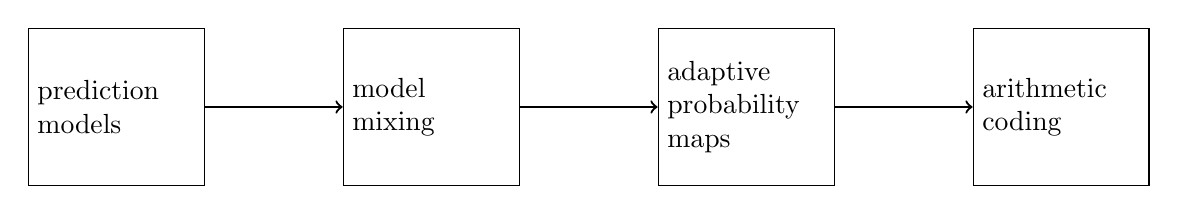
\begin{tikzpicture}[]
	\node[rectangle,draw,minimum height=2cm,text width=2cm] (predModel) at (0,0) {prediction models};
	\node[rectangle,draw,text width=2cm,minimum height=2cm] (modelMix) at (4,0) {model \\ mixing};
	\node[rectangle,draw,text width=2cm,minimum height=2cm] (apm) at (8,0) {adaptive probability maps};
	\node[rectangle,draw,text width=2cm,minimum height=2cm] (arithCoding) at (12,0) {arithmetic coding};

\draw[->,thick](predModel) -- (modelMix);
\draw[->,thick](modelMix) -- (apm);
\draw[->,thick](apm) -- (arithCoding);

\end{tikzpicture}
		}
		\caption{PAQ8 Architecture}
	\end{figure}
	}

	

\end{frame}


\subsection{Model Mixer}
\begin{frame}{Neural Network}
	\begin{alertblock}{Layers of a neural Network}<1->
		A layer, in the context of a neural network, is a \defText{group of neurons}, which take an \defText{input} and provide and \defText{output}. 
	\end{alertblock}
	

	
	
	%Change picture to just a neuron
	\visible<3->{
	\begin{figure}[H]
		\centering
		\resizebox{0.35\textwidth}{!}{
			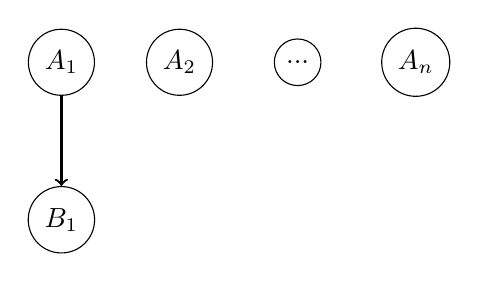
\begin{tikzpicture}[]
	\node[circle,draw] (a1) at (0,0) {$A_1$};
	\node[circle,draw] (a2) at (1.5,0) {$A_2$};
	\node[circle ,draw] (adot) at (3,0) {$...$};
	\node[circle,draw] (an) at (4.5,0) {$A_n$};
	\node[circle,draw] (b1) at (0,-2) {$B_1$};

\draw [->, thick](a1) -- (b1);

\end{tikzpicture}
		}
		\caption{Neural network architecture}
	\end{figure}
	}

\end{frame}

\begin{frame}{Neural Network}
		
	\begin{alertblock}{Neurons of a neural Network}<1->
	A \defText{neuron} takes one or more \defText{inputs} and gives an \defText{output}. \\
	Within the topic of machine learning, the neuron can be understood as a \defText{function}.
	\end{alertblock}

	\visible<2->{
		\begin{figure}[H]
			\centering
			\resizebox{0.35\textwidth}{!}{
				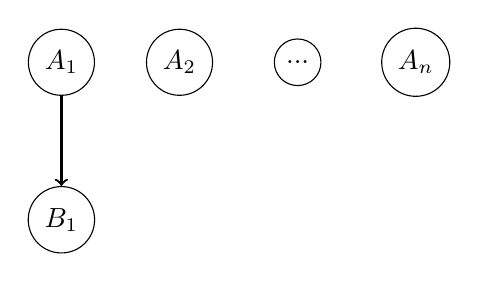
\begin{tikzpicture}[]
	\node[circle,draw] (a1) at (0,0) {$A_1$};
	\node[circle,draw] (a2) at (1.5,0) {$A_2$};
	\node[circle ,draw] (adot) at (3,0) {$...$};
	\node[circle,draw] (an) at (4.5,0) {$A_n$};
	\node[circle,draw] (b1) at (0,-2) {$B_1$};

\draw [->, thick](a1) -- (b1);

\end{tikzpicture}
			}
			\caption{Neural network architecture}
		\end{figure}
	}	
	
\end{frame}


\begin{frame}{Model Mixer}
	\begin{exampleblock}{Model Mixer of paq8l}<1->
		\begin{itemize}
			\item Resembles a neural network with one hidden layer
			\item Hidden layer is between input and output layer\\
			$\hookrightarrow$ Artificial neurons take a set of weighted inputs\\
			Output is produced through activation function
		\end{itemize}
	\end{exampleblock}
	
	\begin{block}{Differences between paq8l and neural networks}<2->
		\begin{enumerate}
			\item Weights for first and second layers are learned online and independently for all nodes:
			\begin{itemize}
				\item Each node trained separately 
				\item reduces predictive cross-entropy error (unlike back propagation)
			\end{itemize}	
			\item Hidden nodes are partitioned into seven sets		 
		\end{enumerate}
	\end{block}
\end{frame}

\subsection{Mixture of Experts}
\subsection{Updating \& Filtering}
\section{Applications for PAQ8}
\section{References}





\end{document}